\documentclass[11pt,letterpaper]{article}
\usepackage[top=0.85in,bottom=0.85in,left=0.8in,right=0.8in]{geometry}
\usepackage{times}
\usepackage{amsmath,amssymb}
\usepackage{booktabs}
\usepackage{graphicx}
\usepackage{enumitem}
\usepackage{titlesec}
\usepackage{caption}
\usepackage{xcolor}
\usepackage[colorlinks=true,linkcolor=blue!50!black,citecolor=blue!50!black,urlcolor=blue!50!black]{hyperref}

\titleformat{\section}{\normalfont\large\bfseries}{\thesection.}{0.5em}{}
\titleformat{\subsection}{\normalfont\normalsize\bfseries}{\thesubsection}{0.6em}{}
\titlespacing*{\section}{0pt}{0.7ex plus .2ex}{0.3ex}
\titlespacing*{\subsection}{0pt}{0.6ex plus .2ex}{0.2ex}
\captionsetup{font=small,labelfont=bf,skip=2pt}
\setlength{\parindent}{1em}
\setlength{\parskip}{0pt}
\setlist{nosep,leftmargin=*}
\setlength{\abovedisplayskip}{3pt}\setlength{\belowdisplayskip}{3pt}
\setlength{\abovedisplayshortskip}{1pt}\setlength{\belowdisplayshortskip}{1pt}
\setlength{\textfloatsep}{6pt plus 2pt}
\setlength{\floatsep}{5pt plus 2pt}
\setlength{\intextsep}{5pt plus 2pt}
\renewcommand{\arraystretch}{0.95}

\newenvironment{prop}[1]{\par\vspace{2pt}\noindent\textbf{Proposition #1.}\itshape\ }{\par\vspace{2pt}}
\newenvironment{lem}[1]{\par\smallskip\noindent\textbf{Lemma #1.}\itshape\ }{\par\smallskip}
\newcommand{\pf}{\noindent\textit{Proof.}\ }
\newcommand{\qedbox}{\hfill$\square$}
\newcommand{\E}{\mathbb{E}}
\newcommand{\abar}{\bar\alpha}
\newcommand{\lstar}{\lambda^{*}}

\begin{document}

\begin{center}
{\LARGE\bfseries When Acceptance Varies: Optimal and Adaptive Speculation\\[2pt] Length in Speculative Decoding}\\[6pt]
{\large Tanish Garg\,$^{*}$ (2401010473) \quad Ananya Soni (2401010068) \quad Rishihood University}\\[3pt]
{\itshape PRISM 2026 --- categories: deconstruction, new variability and simulation}
\end{center}

\begingroup\renewcommand\thefootnote{$*$}
\footnotetext{All numerical results come from the code described in Section~4 (Apple M3, 8\,GB, PyTorch MPS; runs of 10--11 November 2026).}
\endgroup

\vspace{-8pt}
\begin{quote}\small
\textbf{Abstract.} Speculative decoding lets a small draft model guess $\gamma$ tokens that a large model verifies in one pass, with a rejection rule that leaves the output distribution exactly unchanged. The landmark analysis of Leviathan, Kalman and Matias assumes a constant acceptance rate $\alpha$, giving $(1-\alpha^{\gamma+1})/(1-\alpha)$ tokens per pass. We re-derive it, show that speculation helps if and only if $\alpha$ exceeds the cost ratio $c$, and give the optimal $\gamma$ in closed form via the Lambert $W$ function. Letting $\alpha$ vary, we show that the landmark formula is a \emph{lower} bound when difficulty persists for whole rounds (Jensen) and an \emph{upper} bound, a harmonic mean, when it persists at the token level, because rounds start where guesses fail. A threshold rule, draft while the survival probability exceeds $\lstar c$, is throughput-optimal. On GPT-2 traces, acceptance varies widely but persists only briefly, so the formula is accurate to within 1.7\%. An oracle adaptive rule gains 3.8--7.5\%, but calibrated draft confidence recovers only 11--35\% of that, and on a laptop the measured verification cost shrinks all speedups to 1.07--1.19$\times$.
\end{quote}

\section{Introduction}
A large language model writes one token per forward pass, and each pass is dominated by loading weights from memory, so checking several tokens in one pass costs about as much as generating one. Leviathan, Kalman and Matias~\cite{leviathan}, and independently Chen et al.~\cite{chen}, used this to build \emph{speculative decoding}: a small draft model (a fast ``System~1'') guesses $\gamma$ tokens, the large target (a careful ``System~2'') verifies them at once, and a rejection rule keeps the output \emph{exactly} the target's, with 2--3$\times$ speedups on T5-XXL. Their analysis assumes one constant acceptance rate $\alpha$ and picks one $\gamma$. Real text is not uniformly predictable, and acceptance differs by task~\cite{abdellatif}. A fixed $\gamma$ is known to be suboptimal~\cite{disco}, the optimal stopping rule is a threshold~\cite{specdecpp}, and learned policies go further~\cite{l2d}. We ask, at the level of the original formulas: \emph{is the landmark formula still right when $\alpha$ varies, and how much is adapting $\gamma$ worth?} We contribute (i) a re-derivation of the exactness proof and speedup formula; (ii) the condition $\alpha>c$ and a Lambert-$W$ closed form for the optimal $\gamma$; (iii) a two-sided bound on the formula under round-level and token-level persistence; and (iv) a renewal-reward derivation of the threshold rule, tested in simulation and on GPT-2.

\section{Notations and Assumptions}
\noindent\textbf{Notation}\par\smallskip
{\small\centering
\begin{tabular}{@{}ll@{\qquad}ll@{}}
$M_p,\ p$ & target model, next-token distribution & $\gamma$ & draft tokens per round\\
$M_q,\ q$ & draft model, next-token distribution & $c$ & time of one $M_q$ step $\div$ one $M_p$ step\\
$\beta$ & acceptance at one position, $\sum_x\min(p,q)$ & $N,\ T$ & tokens and time ($M_p$ steps) per round\\
$\alpha$ & acceptance rate, $\alpha=\E[\beta]$ & $S(\gamma)$ & speedup, $\E[N]/T$\\
$\abar,\ \sigma^2$ & mean, variance of a random $\alpha$ & $g(\alpha)$ & $\sum_{k=0}^{\gamma}\alpha^k$\\
$A_k$ & probability the first $k$ drafts survive & $\lstar$ & best achievable throughput\\
\end{tabular}\par}

\smallskip\noindent\textbf{Assumptions}
\begin{enumerate}
\item[(A1)] Landmark model: acceptance events in a round are independent, each with probability $\alpha$.
\item[(A1$'$)] Round-level persistence: each round draws its own $\alpha\in[0,1]$ (mean $\abar$, variance $\sigma^2$), independently of the past; within the round, drafts are accepted independently with that $\alpha$.
\item[(A1$''$)] Token-level persistence: the text consists of long stretches; a stretch at level $\alpha$ makes up a share $w(\alpha)$ of all tokens.
\item[(A2)] One target pass over $\gamma+1$ positions costs one target step, so $T=\gamma c+1$ (relaxed in Section~5.2). Sampling is at temperature 1.
\end{enumerate}

\section{Proposed Model and Technique}
\subsection{The landmark result, re-derived}
\begin{lem}{1 (\cite{leviathan,chen})}
Draw $x\sim q$; accept it with probability $\min(1,p/q)$, else draw from $r=\max(0,p-q)/(1-\beta)$. The output is then distributed exactly as $p$, and
\begin{equation}
\Pr[\text{accept}]=\beta=\textstyle\sum_x\min(p(x),q(x))=1-\tfrac12\lVert p-q\rVert_1 .
\end{equation}
\end{lem}
\pf The output is $x$ by acceptance, with probability $q(x)\min(1,p(x)/q(x))=\min(p,q)$, or by rejection then resampling, with probability $(1-\beta)r(x)=\max(0,p-q)$; the sum is $p$. As $\sum\max(0,p-q)=1-\beta$, $r$ is a distribution. By the chain rule the whole text follows $M_p$.\qedbox

\smallskip
Under (A1), $\Pr[N\ge n+1]=\alpha^n$ for $n\le\gamma$, so the tail-sum formula and a geometric series give
\begin{equation}
\E[N]=\sum_{n=0}^{\gamma}\alpha^n=\frac{1-\alpha^{\gamma+1}}{1-\alpha},\qquad S(\gamma)=\frac{1-\alpha^{\gamma+1}}{(1-\alpha)(\gamma c+1)} .
\end{equation}

\subsection{The best fixed $\gamma$}
\begin{prop}{1}
Under (A1)--(A2): (a) $S$ is quasi-concave in $\gamma$; (b) some $\gamma\ge1$ beats $\gamma=0$ if and only if $\alpha>c$; (c) the real maximiser is
\begin{equation}
\gamma^{*}=\frac{y-L-c}{Lc},\qquad L=-\ln\alpha,\qquad y=-c\,W_{-1}\!\left(-e^{-1-L(1/c-1)}\right).
\end{equation}
\end{prop}
\pf (a) The numerator of $S$ is positive, increasing and concave, and the denominator is positive and affine, so $\{S\ge t\}=\{\text{num}-t\cdot\text{den}\ge0\}$ is an interval. (b) $S(1)/S(0)=(1+\alpha)/(1+c)$; if $S(1)\le S(0)$, quasi-concavity forces $S(\gamma)\le S(0)$ for all $\gamma\ge1$. (c) With $u=\alpha^{\gamma+1}$, $S'=0$ gives $Lu(\gamma c+1)=c(1-u)$. Putting $y=L(\gamma c+1)+c$ gives $u=c/y$ and $(y/c)e^{-y/c}=e^{-1-L(1/c-1)}$, a Lambert-$W$ equation~\cite{corless}. Since $y>c$, $-y/c<-1$, which selects the branch $W_{-1}$.\qedbox

\subsection{Variable acceptance cuts both ways}
\begin{prop}{2 (round-level persistence)}
Under (A1$'$), for every fixed $\gamma$,
\begin{equation}
\E[N]=\sum_{k=0}^{\gamma}\E[\alpha^k]\ \ge\ g(\abar),\qquad \E[N]-g(\abar)\approx\sigma^2\sum_{k=2}^{\gamma}\binom{k}{2}\abar^{\,k-2}.
\end{equation}
\end{prop}
\pf Given $\alpha$, (2) gives $\E[N\mid\alpha]=g(\alpha)$. Average over $\alpha$ and apply Jensen's inequality~\cite{jensen} to the convex maps $x^k$ ($k\ge2$) on $[0,1]$. The approximation is the second-order Taylor term of each $x^k$ at $\abar$.\qedbox

\smallskip
If instead each token draws an independent $\alpha_j$, then $\E[\alpha_1\cdots\alpha_k]=\abar^k$ and (2) is exact: variability alone does nothing; persistence matters.

\begin{prop}{2$'$ (token-level persistence)}
Under (A1$''$), with a fixed $\gamma$, the mean number of tokens per round is a harmonic mean, and
\begin{equation}
\bar N_{\text{round}}=\Big(\E_w\big[1/g(\alpha)\big]\Big)^{-1}\ \le\ g(\abar)\ \le\ \E_w\big[g(\alpha)\big].
\end{equation}
\end{prop}
\pf By the renewal theorem, a stretch of $\ell$ tokens at level $\alpha$ is covered by about $\ell/g(\alpha)$ rounds, so rounds fall in level $\alpha$ in proportion to $w(\alpha)/g(\alpha)$, and the per-round mean of $N$ is $\sum w/\sum(w/g)$. Next, $(1/g)''=(2g'^2-g\,g'')/g^3$, and $2g'^2-g\,g''$ is a polynomial in $\alpha$ whose coefficients we computed exactly to be non-negative for every $\gamma\le60$. Hence $1/g$ is convex on $[0,1]$, and Jensen gives $\E_w[1/g]\ge1/g(\abar)$. The right inequality is Proposition~2.\qedbox

\smallskip
Intuition: rounds start right after rejections, which happen in hard text, so a random \emph{round} is more often hard than a random \emph{token} (the inspection paradox~\cite{ross}).

\subsection{The throughput-optimal adaptive rule}
\begin{prop}{3}
If System~1 knows the non-increasing survival probabilities $A_k$ before drafting, the throughput-optimal policy drafts token $k$ if and only if
\begin{equation}
A_k\ \ge\ \lstar c,\qquad \lstar=\max_\pi \E[N_\pi]/\E[T_\pi].
\end{equation}
\end{prop}
\pf By the renewal-reward theorem~\cite{ross}, long-run throughput is $\E[N]/\E[T]$. By Dinkelbach's lemma~\cite{dinkelbach}, a policy maximises this ratio if and only if it maximises $\E[N-\lstar T]$, which separates by round. Given the information, $\E[N]=\sum_{k\le\gamma}A_k$, so adding draft $k$ changes the objective by $A_k-\lstar c$. As $A_k$ is non-increasing, the optimum is the largest $k$ with $A_k\ge\lstar c$.\qedbox

\smallskip
Under (A1$'$), $\gamma(\alpha)=\lfloor\ln(\lstar c)/\ln\alpha\rfloor$. The threshold form is proved for an MDP in~\cite{specdecpp}; our route shows that $\lstar c$ is the \emph{opportunity cost} of one draft step, and since a fixed $\gamma$ is admissible, (6) never does worse.

\section{Solution Procedure}
\textbf{Algorithm (adaptive System~1).} (1) Fit $\lstar$ by fixed-point iteration (run the rule, set $\lambda$ to tokens $\div$ time, repeat). (2) Each round, estimate $A_k$ from the round's $\alpha$, the regime, or calibrated draft confidence. (3) Draft while $A_k\ge\lstar c$ (cap 40). (4) Verify with one $M_p$ pass (Lemma~1).

\textbf{Experiments.} \emph{E0} checks every formula against simulation or exact enumeration: all 38 checks pass (output law vs.\ $p$: $5.6\times10^{-17}$; (3) vs.\ grid search: four decimals). \emph{E1} evaluates (2)--(3) over $(\alpha,c)$. \emph{E2} varies $\alpha$: (A) $\alpha\sim\mathrm{Beta}(\abar\kappa,(1-\abar)\kappa)$ per round, computed exactly; (B) the same per token; (C) two Markov regimes ($\alpha=0.95/0.4$) switching after each token with probability $s$; (D) Model~A with a noisy estimate $\hat\alpha=\alpha+\mathcal N(0,\sigma^2)$; we use $\abar=0.7$, $c=0.05$ and 5 seeds. \emph{E3} uses distilgpt2 (82M)~\cite{distil} as the draft and gpt2-large (774M) or gpt2-medium (355M)~\cite{gpt2} as the target, on 100 passages each of prose (WikiText-2~\cite{wikitext}), maths (GSM8K~\cite{gsm8k}) and code (HumanEval~\cite{humaneval}), 128 tokens each. One forward pass per model records $\beta_t$ along the reference text; the traces are replayed through a round simulator, with $\lstar$, the calibrator (isotonic or logistic regression from draft confidence to $\beta$) and the best fixed $\gamma$ fitted on half the passages and tested on the rest.

\textbf{Worked example.} With $\alpha=0.8$ and $c=0.05$: $L=0.2231$, $L(1/c-1)=4.240$, $W_{-1}(-e^{-5.240})=W_{-1}(-0.00530)=-7.217$, $y=0.3609$, and $\gamma^*=(0.3609-0.2231-0.05)/(0.2231\cdot0.05)=7.86$. Since $S(7)=3.082<S(8)=3.092$, take $\gamma=8$: each round yields $(1-0.8^9)/0.2=4.33$ tokens in $1.4$ target steps, a $3.09\times$ speedup. If $\alpha$ varies between rounds (mean 0.7, SD 0.138), $\lstar=2.877$, so $\lstar c=0.144$: the rule drafts 37 tokens at $\alpha=0.95$, 5 at $0.7$, 2 at $0.5$ and none at $0.1$, reaching 2.877 against 2.556 for the best fixed $\gamma$. With half the tokens at $\alpha=0.95$ and half at $0.4$ ($\gamma=5$), the harmonic mean $2/(\tfrac1{5.30}+\tfrac1{1.66})=2.53$ is below $g(0.675)=2.79$.

\section{Results}
\subsection{Simulation}
\begin{figure}[t]
\centering
\begin{minipage}[t]{0.47\linewidth}\centering
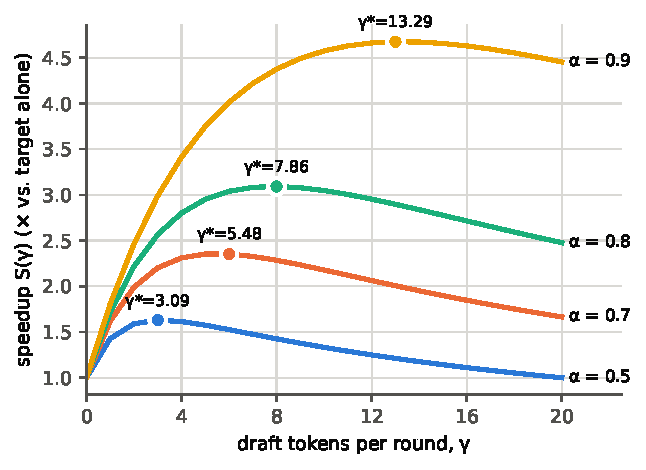
\includegraphics[width=0.82\linewidth]{figures/fig1_speedup_curves.pdf}\\[-1pt]{\small (a) $S(\gamma)$ under (A1), $c=0.05$}
\end{minipage}\hfill
\begin{minipage}[t]{0.47\linewidth}\centering
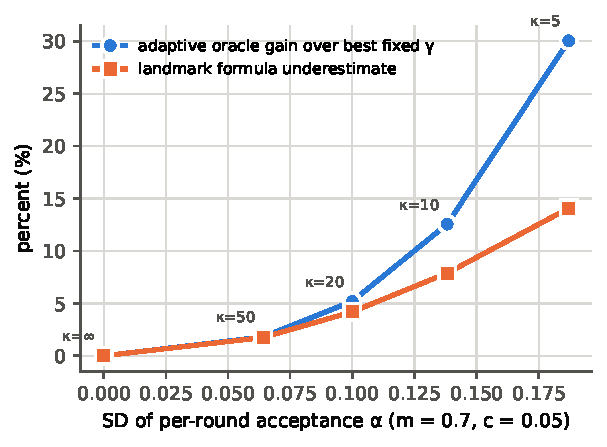
\includegraphics[width=0.82\linewidth]{figures/fig3_variability_gain.pdf}\\[-1pt]{\small (b) Model A: adaptive gain, landmark error}
\end{minipage}
\caption{(a) Speedup is quasi-concave in $\gamma$, and higher acceptance moves the peak to longer drafts. (b) Under round-level persistence, the gain from adapting $\gamma$ and the landmark formula's underestimate both grow faster than linearly in SD$(\alpha)$ (exact computation, $\abar=0.7$, $c=0.05$).}
\end{figure}

\begin{table}[t]
\centering\small
\caption{Left: token-level persistence (Model C). The landmark at $\abar=0.675$, $\gamma=5$ gives 2.229; the harmonic bound (5) gives 2.022 ($-9.3\%$). Right: noisy System~1 (Model D, SD$(\alpha)=0.138$): share of the oracle gain ($2.556\to2.877$) kept using the raw $\hat\alpha$ or its posterior mean.}
\begin{tabular}{@{}ccccc@{\qquad}ccc@{}}
\toprule
$s$ & Best fixed (vs.\ landmark) & Hard starts & Naive $A_k=\alpha^k$ & Correct $A_k$ & $\sigma$ & Raw $\hat\alpha$ & Posterior\\
\midrule
0.01 & 2.043 ($-8.3\%$) & 75.3\% & +10.6\% & +13.8\% & 0.05 & 72\% & 75\%\\
0.05 & 2.062 ($-7.5\%$) & 74.3\% & +2.6\% & +11.8\% & 0.10 & 19\% & 46\%\\
0.20 & 2.121 ($-4.8\%$) & 68.9\% & $-19.1\%$ & +5.3\% & 0.20 & $-79\%$ & 13\%\\
\bottomrule
\end{tabular}
\end{table}

(1) \emph{Under round-level persistence the landmark formula is biased low}: by 1.7, 4.2, 7.9 and 14.1\% at SD$(\alpha)=0.064$--$0.19$, each within one point of the second-order term in (4). The best fixed $\gamma$ drifts from 6 to 10, and adaptivity gains 1.8--30\% (Figure~1b). With per-token independent $\alpha$ (Model B), the formula is exact to 0.06\%. (2) \emph{Token-level persistence reverses the sign} (Table~1): the formula overestimates by 4.8--8.3\%, and the simulation lies between the harmonic bound and the landmark; only half the tokens are hard, but 69--75\% of rounds start in hard text. (3) \emph{The rule needs the right $A_k$}: assuming the regime lasts all round loses 19.1\% under fast switching, while the correct $A_k$ gains 5--14\% at every $s$. (4) \emph{Calibration is the bottleneck}: a raw estimate with error SD 0.2 is worse than a fixed $\gamma$, but its posterior mean never is.

\subsection{GPT-2 measurements}
Per-token times are 5.9\,ms (draft), 24.0\,ms (gpt2-medium) and 47.7\,ms (gpt2-large), so $c=0.245$ and $0.123$. \begin{table}[t]
\centering\footnotesize\setlength{\tabcolsep}{4pt}
\caption{GPT-2 results on the test half (5 replay seeds, SD $\le0.015$; throughput in tokens per target step). ``Real vs.\ ctrl'' compares replay with real $\beta_t$ against a control with $\beta_t$ held at its mean, at the landmark $\gamma$ (3 for large, 2 for medium). Under (A2) the landmark $\gamma$ is the best fixed $\gamma$; gains are over it. Wall-clock uses $T=\gamma c+v(\gamma+1)$ with the measured verify ratio $v$ ($v(9)\approx1.70$ large, $1.34$ medium).}
\begin{tabular}{@{}llcccc@{\quad}cccc@{\quad}cc@{}}
\toprule
& & \multicolumn{4}{c}{Acceptance $\beta_t$} & \multicolumn{4}{c}{Throughput under (A2)} & \multicolumn{2}{c}{Wall-clock}\\
\cmidrule(lr){3-6}\cmidrule(lr){7-10}\cmidrule(l){11-12}
Target & Text & Mean & SD & ACF 1/5 & Real vs.\ ctrl & Best fixed & Calibrated & Oracle & Recovered & Best fixed ($\gamma$) & Oracle\\
\midrule
large & prose & 0.590 & 0.210 & .21/.04 & $-0.6\%$ & 1.556 & +1.1\% & +4.2\% & 26\% & 1.066 (4) & 1.135\\
large & maths & 0.601 & 0.236 & .18/.09 & $-1.2\%$ & 1.582 & +1.5\% & +5.8\% & 26\% & 1.086 (4) & 1.152\\
large & code & 0.604 & 0.270 & .20/.11 & $-1.4\%$ & 1.602 & +2.6\% & +7.5\% & 35\% & 1.106 (4) & 1.200\\
medium & prose & 0.613 & 0.193 & .19/.03 & $-0.4\%$ & 1.329 & +0.4\% & +3.8\% & 11\% & 1.162 (2) & 1.214\\
medium & maths & 0.627 & 0.217 & .16/.09 & $-0.7\%$ & 1.354 & +0.8\% & +5.6\% & 14\% & 1.184 (2) & 1.264\\
medium & code & 0.628 & 0.251 & .23/.08 & $-1.0\%$ & 1.357 & +1.9\% & +7.5\% & 25\% & 1.186 (2) & 1.300\\
\bottomrule
\end{tabular}
\end{table}

(5) \emph{Acceptance is highly variable but only briefly persistent} (Table~2): SD 0.19--0.27, with 19\% of code positions above 0.9, yet lag-1 autocorrelation is about 0.2 and nearly gone by lag 5. (6) \emph{The landmark formula is slightly optimistic}: real $\beta$ gives 0.4--1.4\% less than the constant-$\beta$ control in all six cells, as Proposition 2$'$ (not 2) predicts. The effect is small, so under (A2) the landmark $\gamma$ is the best fixed $\gamma$ in every cell. (7) \emph{Adaptivity has value, but draft confidence captures little of it}: an oracle gains 3.8--7.5\% (most on code), and calibrated confidence recovers 11--35\% of that, in line with Model D. (8) \emph{Verification is not free on a laptop}: a block costs 1.3--1.7 target steps, rising mostly from $m=1$ to $2$, consistent with~\cite{chordiya}. Speedups shrink to 1.07--1.19$\times$ (never below 1), and the best fixed $\gamma$ for gpt2-large rises from 3 to 4. These timings are noisy (under 1.5\,GB free memory; non-monotone $v(m)$).

\section{Conclusion and Future Scope}
\textbf{Conclusion.} Speculative decoding is exact because $\min(p,q)+\max(0,p-q)=p$. Under constant acceptance, speculation helps exactly when $\alpha>c$, with a Lambert-$W$ optimal length. When acceptance varies, \emph{how long difficulty persists} sets the sign of the formula's error: round-level persistence makes it pessimistic (Jensen), token-level persistence optimistic (a harmonic mean, because rounds begin where guesses fail); on GPT-2 the two nearly cancel. The rule $A_k\ge\lstar c$ is worth 4--8\% with perfect knowledge, but draft confidence captures about a quarter: a cheap, calibrated System~1 is the real open problem.

\textbf{Limitations.} (A1$'$), (A1$''$) are idealised extremes; timings come from one 8\,GB laptop; the models are small; adaptive length itself is not new~\cite{disco,specdecpp,l2d}. \textbf{Future scope:} convexity for all $\gamma$, Markov acceptance, and a learned acceptance predictor.

\newpage
\begin{thebibliography}{99}\small
\setlength{\itemsep}{2pt}
\bibitem{leviathan} Y. Leviathan, M. Kalman and Y. Matias, ``Fast inference from Transformers via speculative decoding,'' in \emph{Proc.\ 40th Int.\ Conf.\ on Machine Learning (ICML)}, PMLR vol.~202, pp.~19274--19286, 2023.
\bibitem{chen} C. Chen, S. Borgeaud, G. Irving, J.-B. Lespiau, L. Sifre and J. Jumper, ``Accelerating large language model decoding with speculative sampling,'' arXiv:2302.01318, 2023.
\bibitem{disco} J. Mamou, O. Pereg, D. Korat, M. Berchansky, N. Timor, M. Wasserblat and R. Schwartz, ``Dynamic speculation lookahead accelerates speculative decoding of large language models,'' in \emph{Proc.\ 4th NeurIPS Efficient Natural Language and Speech Processing Workshop}, PMLR vol.~262, pp.~456--467, 2024.
\bibitem{specdecpp} K. Huang, X. Guo and M. Wang, ``SpecDec++: Boosting speculative decoding via adaptive candidate lengths,'' in \emph{Conf.\ on Language Modeling (COLM)}, 2025. arXiv:2405.19715.
\bibitem{l2d} J. Zhang et al., ``Learning to draft: Adaptive speculative decoding with reinforcement learning,'' in \emph{Int.\ Conf.\ on Learning Representations (ICLR)}, 2026. arXiv:2603.01639.
\bibitem{abdellatif} S. Abdellatif, ``Acceptance dynamics across cognitive domains in speculative decoding,'' arXiv:2604.14682, 2026.
\bibitem{chordiya} P. Chordiya, ``Lossless but not free: An empirical anatomy of speculative decoding on consumer hardware,'' arXiv:2607.17283, 2026.
\bibitem{dinkelbach} W. Dinkelbach, ``On nonlinear fractional programming,'' \emph{Management Science}, vol.~13, no.~7, pp.~492--498, 1967.
\bibitem{corless} R. M. Corless, G. H. Gonnet, D. E. G. Hare, D. J. Jeffrey and D. E. Knuth, ``On the Lambert W function,'' \emph{Advances in Computational Mathematics}, vol.~5, pp.~329--359, 1996.
\bibitem{jensen} J. L. W. V. Jensen, ``Sur les fonctions convexes et les in\'egalit\'es entre les valeurs moyennes,'' \emph{Acta Mathematica}, vol.~30, pp.~175--193, 1906.
\bibitem{ross} S. M. Ross, \emph{Stochastic Processes}, 2nd ed., Wiley, 1996.
\bibitem{gpt2} A. Radford, J. Wu, R. Child, D. Luan, D. Amodei and I. Sutskever, ``Language models are unsupervised multitask learners,'' OpenAI technical report, 2019.
\bibitem{distil} V. Sanh, L. Debut, J. Chaumond and T. Wolf, ``DistilBERT, a distilled version of BERT: smaller, faster, cheaper and lighter,'' arXiv:1910.01108, 2019.
\bibitem{wikitext} S. Merity, C. Xiong, J. Bradbury and R. Socher, ``Pointer sentinel mixture models,'' in \emph{Int.\ Conf.\ on Learning Representations (ICLR)}, 2017.
\bibitem{gsm8k} K. Cobbe et al., ``Training verifiers to solve math word problems,'' arXiv:2110.14168, 2021.
\bibitem{humaneval} M. Chen et al., ``Evaluating large language models trained on code,'' arXiv:2107.03374, 2021.
\end{thebibliography}

\end{document}
